%%%%%%%%%%%%%%%%%%%%%%%%
\section{Nonlocal Allen-Cahn energy}
%%%%%%%%%%%%%%%%%%%%%%%%
\label{Sec:Nonlocal_AllenCahn_Energy}




This section is devoted to the energy functional associated to the Allen-Cahn equation. We first define appropriately the functional spaces where we are going to apply classic techniques of calculus of variations. We also rewrite the energy in terms of the new kernel $\overline{K}$ and finally, we establish a sharp energy estimate. Through all the section we follow the notation of \cite{CozziPassalacqua}.



Let us start by defining the functional spaces that we are going to consider in this paper. Given a set $\Omega \subset \R^n$ and a translation invariant and positive kernel $K$ satisfying \eqref{Eq:Symmetry&IntegrabilityOfK}, we define the space
$$
\H^K(\Omega) := \setcond{w \in L^2(\Omega)}{[w]^2_{\H^K(\Omega)} < + \infty},
$$
where
$$
[w]^2_{\H^K(\Omega)} := \dfrac{1}{2}\int\int_{\R^{2n} \setminus (\R^n\setminus\Omega)^2} |w(x) - w(y)|^2 K(x-y) \d x \d y\,.
$$
We also define
\begin{align*}
	\H^K_0(\Omega) &:= \setcond{w \in \H^K(\Omega)}{ w = 0 \quad \textrm{a.e. in } \R^n \setminus \Omega} \\
	&\ = \setcond{w \in \H^K(\R^n)}{ w = 0 \quad \textrm{a.e. in } \R^n \setminus \Omega}.
\end{align*}

Assume that $\Omega \subset \R^{2m}$ is a domain of double revolution. Then, we define
$$
\widetilde{\H}^K(\Omega) := \setcond{w \in \H^K(\Omega)}{w \textrm{ is doubly radial a.e.}}.
$$
and
$$
\widetilde{\H}^K_0(\Omega) := \setcond{w \in \H^K_0(\Omega)}{w \textrm{ is doubly radial a.e.}}.
$$
We will add the subscript `odd' and `even' to these spaces to consider only functions that are odd (respectively even) with respect to the Simons cone.


\begin{remark}
\label{Remark:DecompositionHK}
If $\widetilde{\H}^K_0(\Omega)$ is equipped with the scalar product
$$
\langle v,w \rangle_{\widetilde{\H}^K_0(\Omega)} := \dfrac{1}{2}\int_{\R^{2m}} \int_{\R^{2m}}  \big(v(x) - v(y)\big)\big(w(x) - w(y)\big) K(x-y) \d x \d y\,,
$$
then, it is easy to check that $\widetilde{\H}^K_0(\Omega)$ can be decomposed as the orthogonal
direct sum of $\widetilde{\H}^K_{0,\, \mathrm{even}}(\Omega)$ and $\widetilde{\H}^K_{0,\,
\mathrm{odd}}(\Omega)$.
\end{remark}

Note that when $K$ satisfies \eqref{Eq:Ellipticity}, then $\H^K_0 (\Omega) = \H^\s_0 (\Omega)$,
which is the space associated to the kernel of the fractional Laplacian, $K(y) = |y|^{-n-2\s}$.
Furthermore, $\H^\s(\Omega) \subset H^\s(\Omega)$, the usual fractional Sobolev space (see
\cite{HitchhikerGuide}).  For more comments on this, see~\cite{CozziPassalacqua}.

Once presented the functional setting of our problem, we define now  the energy functional associated to the Allen-Cahn equation. 

\begin{definition}
	Given a kernel $K$ satisfying \eqref{Eq:Symmetry&IntegrabilityOfK}, a potential $G$ and a function $w\in \H^K(\Omega)$, with $\Omega\subset \R^{n}$, we define the \emph{nonlocal Allen-Cahn energy} by
	$$
	\ecal(w, \Omega) := \ecal_\mathrm{K}(w,\Omega) + \ecal_\mathrm{P}(w,\Omega)\,,
	$$
	where
	$$
	\ecal_\mathrm{K}(w, \Omega) := \dfrac{1}{2} [w]^2_{\H^K(\Omega)} \quad \text{ and } \quad  \ecal_\mathrm{P}(w, \Omega) := \int_{\Omega} G(w)
	\,.
	$$
	We will call $\ecal_\mathrm{K}$ and $\ecal_\mathrm{P}$ the \emph{kinetic} and \emph{potential} energy respectively.
\end{definition}


For short, we will denote $\ecal(w, \R^n) =: \ecal(w)$. Note that, for functions $w\in \H^K_0(\Omega)$, $\ecal_\mathrm{K}(w,\Omega) = \ecal_\mathrm{K}(w)$. Moreover, if $G\geq 0$, the energy satisfies $
\ecal(w, \Omega) \leq \ecal(w, \Omega')$  whenever $ \Omega \subset \Omega'$.

Sometimes is it useful to rewrite the kinetic energy as
\begin{equation}
	\label{Eq:KineticEnergyInteractions}
	\begin{split}
	\ecal_\mathrm{K}(w, \Omega) := \dfrac{1}{4} \int_\Omega \int_\Omega |w(x) - w(y)|^2 K(x-y) \d x \d y \qquad \qquad \\
	+ \dfrac{1}{2} \int_\Omega \int_{\R^n \setminus \Omega} |w(x) - w(y)|^2 K(x-y) \d x \d y\,.
	\end{split}	
\end{equation}
Roughly speaking, we have split the kinetic energy into ``interactions inside-inside'' and ``interactions inside-outside''. Our goal is, as in the previous section, rewrite the energy in terms of the doubly radial kernel $\overline{K}$ and with integrals only computed in $\ocal$. In particular, we are interested in finding a suitable expression similar to \eqref{Eq:KineticEnergyInteractions} for the kinetic energy. To do this, we introduce the following notation for the interaction. For $A$, $B\subset \ocal$ of double revolution, we define
\begin{equation}
	\label{Eq:DefIw}
	\begin{split}
	I_w(A,B) := \int_A  \int_B  \ |w(x)-w(y)|^2 \left\{ \overline{K}(x,y) - \overline{K}(x,y^\star) \right\} \d x \d y  \\
	+2 \int_A  \int_B  \left\{w^2(x)+w^2(y)\right\} \overline{K}(x,y^\star) \d x \d y\,.
	\end{split}
\end{equation}
Thanks to this notation, we rewrite the kinetic energy as follows.


\begin{lemma}
	\label{Lemma:ShortExpressionEnergy}
Let $\Omega\subset \R^{2m}$ be a domain of double revolution and let $w\in \widetilde{\H}^K_{0,\, \mathrm{odd}}(\Omega)$. Let $K$ be a radially symmetric kernel satisfying \eqref{Eq:Symmetry&IntegrabilityOfK}. Then, 
\begin{align*}
\label{Eq:EnergyOddInOcal2}
\ecal_\mathrm{K}(w, \Omega) = \frac{1}{2} I_w(\Omega\cap\ocal,\Omega\cap\ocal) + I_w(\Omega\cap\ocal,\ocal\setminus\Omega),
\end{align*}
where $I_w(\cdot, \cdot)$ is the interaction defined in \eqref{Eq:DefIw}.
\end{lemma}

\begin{proof}
	
	First, in \eqref{Eq:KineticEnergyInteractions} we consider the change $ y = R\tilde{y}$. Then, since $w$ is doubly radial and $\Omega$ is of double revolution, by taking the average among all $R\in SO(m)^2$ as in Lemma~\ref{Lemma:AlternativeOperatorExpression}, we obtain
	$$
	\ecal_\mathrm{K}(w, \Omega) = \frac{1}{4} \int_{\Omega} \int_{\Omega} |w(x)-w(y)|^2 \overline{K}(x,y) \d x \d y + \frac{1}{2} \int_{\Omega} \int_{\R^n \setminus \Omega} |w(x)-w(y)|^2 \overline{K}(x,y) \d x \d y\,.
	$$
	Now we split $\Omega$ into $\Omega \cap \ocal$ and $\Omega \setminus \ocal$. By using the change of variables given by $(\cdot)^\star$ and the odd symmetry of $w$, we get	
	\begin{align*}
\ecal_\mathrm{K}(w, \Omega) =  & \frac{1}{2} \int_{\Omega\cap \ocal} \int_{\Omega \cap \ocal} |w(x)-w(y)|^2 \overline{K}(x,y) + |w(x)+w(y)|^2 \overline{K}(x,y^\star) \d x \d y  \\
& + \int_{\Omega\cap \ocal} \int_{\ocal \setminus \Omega} |w(x)-w(y)|^2 \overline{K}(x,y) + |w(x)+w(y)|^2 \overline{K}(x,y^\star) \d x \d y  \\
= & \frac{1}{2} \int_{\Omega\cap \ocal} \int_{\Omega \cap \ocal}  \ |w(x)-w(y)|^2 \left\{ \overline{K}(x,y) - \overline{K}(x,y^\star) \right\}  +2 \left\{w^2(x)+w^2(y)\right\} \overline{K}(x,y^\star) \d x \d y\,\\
&+ \int_{\Omega\cap \ocal} \int_{\ocal \setminus \Omega}  \ |w(x)-w(y)|^2 \left\{ \overline{K}(x,y) - \overline{K}(x,y^\star) \right\}  +2 \left\{w^2(x)+w^2(y)\right\} \overline{K}(x,y^\star) \d x \d y\,\\
= & \frac{1}{2} I_w(\Omega\cap\ocal,\Omega\cap\ocal) + I_w(\Omega\cap\ocal,\ocal\setminus\Omega).
\end{align*}
\end{proof}

The following are two lemmas regarding the decrease of the energy under some operations.
\begin{lemma}
\label{Lemma:DecreaseEnergy} 
Let $K$ be a radially symmetric kernel satisfying \eqref{Eq:Symmetry&IntegrabilityOfK} and \eqref{Eq:KernelInequalityReflexion}. Given $u\in\widetilde{\H}^K_{\mathrm{odd}}(\Omega)$, we define
\begin{equation*}
v(x) = \begin{cases}
\hspace{3.2mm}|u(x)| \,\,\, &\text{if } \,\,\, x\in\ocal,\\
-|u(x)| \,\,\, &\text{if } \,\,\, x\in\ical\, ,
\end{cases}
\quad 
\text{ and }
\quad
w(x) = \begin{cases}
\hspace{3.6mm}\min\{1,u(x)\} \,\,\, &\text{if } \,\,\, x\in\ocal,\\
\,\,\,\max\{-1,u(x)\} \,\,\, &\text{if } \,\,\, x\in\ical\,.
\end{cases}
\end{equation*}
Then
$$ \ecal(v,\Omega) \leq \ecal(u,\Omega) \quad 
\text{ and }
\quad \ecal(w,\Omega) \leq \ecal(u,\Omega) \,.  $$
\end{lemma}

\begin{proof}
We first establish the result for $v$. Let us show that  $\ecal_\mathrm{K}(v) = \ecal_\mathrm{K}(u)$. Note that $v\in \widetilde{\H}^K_{\mathrm{odd}}(\Omega)$. Thus, by the expression of the kinetic energy given in Lemma~\ref{Lemma:ShortExpressionEnergy} and the fact that $\overline{K}(x,y) > \overline{K}(x,y^\star)> 0$ if $x,y\in \ocal$ ---see \eqref{Eq:KernelInequalityReflexion}---, we only need to check that $|v(x)-v(y)|^2\leq |u(x)-u(y)|^2$ and $v^2(x)\leq u^2(x)$ whenever $x,y\in\ocal$. The first condition follows from
$$ \big||u(x)|-|u(y)|\big|^2\leq |u(x)-u(y)|^2 \Longleftrightarrow w(x)w(y) \leq |w(x)w(y)|,  
$$
while the second one is trivial and it is in fact an equality. Concerning the potential energy, since $G$ is an even function we have that $\ecal_\mathrm{P}(v) = \ecal_\mathrm{P}(u)$, and therefore we get the desired result for $v$ by adding the kinetic and potential energies.

We show now the result for $w$. Let us show that  $\ecal_\mathrm{K}(w) = \ecal_\mathrm{K}(u)$. As before, $w\in \widetilde{\H}^K_{\mathrm{odd}}(\Omega)$. Thus, we only need to check that $|w(x)-w(y)|^2\leq |u(x)-u(y)|^2$ and $w^2(x) \leq u^2(x)$ whenever $x,y\in\ocal$. The first inequality is trivial whenever $u(x)\leq 1$ and $u(y)\leq 1$, or $u(x)\geq 1$ and $u(y)\geq 1$. If $u(x)\geq 1$ and $u(y)\leq 1$, then $ |u(x)-u(y)|^2-|w(x)-w(y)|^2 = |u(x)-u(y)|^2-|1-u(y)|^2 = (u(x)-1))^2+2(u(x)-1)(1-u(y)) \geq 0$. The second inequality follows from the fact that $w^2(x) = u^2(x)$ when $u(x)\leq 1$, while $w^2(x) = 1 \leq u^2(x)$ if $u(x)\geq 1$. Concerning the potential energy, since $G$ is such that $G(x)\geq G(1) = G(-1) = 0$ if $|x|\leq 1$, then clearly $\ecal_\mathrm{P}(w) \leq \ecal_\mathrm{P}(u)$, and therefore we get the desired result by adding the kinetic and potential energies.
\end{proof}



Next we present a result that will be used later to show that a function $u\in \widetilde{\H}^K_{0}(\Omega)$ that minimizes the nonlocal Allen-Cahn energy, only among odd functions, is actually a weak solution of a semilinear Dirichlet problem in $\Omega$.

\begin{proposition}
	\label{Prop:WeakSolutionForAllTestFunctions}
	Let $\Omega \subset \R^{2m}$ be a bounded set of double revolution and let $L\in \Lr$ with kernel $K$. Let $u\in \widetilde{\H}^K_{0}(\Omega)$ such that
	$$
	\int_{\R^{2m}}\int_{\R^{2m}} \{u(x)-u(y)\}\{\xi(x)-\xi(y)\} K(|x-y|) \d x \d y = \int_{\R^{2m}} f(u(x)) \xi(x) \d x
	$$
	for every $\xi \in C^\infty_0(\Omega)$ that is doubly radial. Then, $u$ is a weak solution of
	$$
	\beqc{\PDEsystem}
	Lu &=& f(u) & \text{in } \Omega\,,\\
	u &=& 0 & \text{in } \R^{2m}\setminus \Omega\,,
	\eeqc
	$$
	i.e.,
	$$
	\int_{\R^{2m}}\int_{\R^{2m}} \{u(x)-u(y)\}\{\eta(x)-\eta(y)\} K(|x-y|) \d x \d y = \int_{\R^{2m}} f(u(x)) \eta(x) \d x
	$$
	for every $\eta \in C^\infty_0(\Omega)$ (not necessarily symmetric).
\end{proposition}

\begin{proof}
	Let $\eta \in C^\infty_0(\Omega)$. Then, given $R\in SO(m)^2$,
	\begin{align*}
	&\int_{\R^{2m}}\int_{\R^{2m}} \{u(x)-u(y)\}\{\eta(x)-\eta(y)\} K(|x-y|) \d x \d y = \\
	%&\quad \quad \quad = \int_{\R^{2m}}\int_{\R^{2m}} \{u(R^{-1}x)-u(R^{-1}y)\}\{\eta(x)-\eta(y)\} K(|x-y|) \d x \d y \\
	&\quad \quad \quad = \int_{\R^{2m}}\int_{\R^{2m}} \{u(x)-u(y)\}\{\eta(R x)-\eta(R y)\} K(|x-y|) \d x \d y\,,
	\end{align*}
	where we have used the change $x = R\tilde{x}$, $y = R \tilde{y}$. Integrating the previous expression with respect to $R$ and taking the average, we get
	\begin{align*}
	& \int_{\R^{2m}}\int_{\R^{2m}} \{u(x)-u(y)\}\{\eta(x)-\eta(y)\} K(|x-y|) \d x \d y = \\
	&\quad \quad \quad =\average_{SO(m)^2} \int_{\R^{2m}}\int_{\R^{2m}} \{u(x)-u(y)\}\{\eta(R x)-\eta(R y)\} K(|x-y|) \d x \d y \d R \\
	%&\quad \quad \quad= \int_{\R^{2m}}\int_{\R^{2m}} \{u(x)-u(y)\}\left \{\average_{SO(m)^2}\eta(R x)\d R-\average_{SO(m)^2} \eta(Ry) \d R \right \} K(|x-y|) \d x \d y \\
	&\quad \quad \quad= \int_{\R^{2m}}\int_{\R^{2m}} \{u(x)-u(y)\}\left \{\overline{\eta}(x) -\overline{\eta}(y)  \right \} K(|x-y|) \d x \d y \,.
	\end{align*}
	Here we have used the notation
	$$
	\overline{\eta}(x) := \average_{SO(m)^2}\eta(R x)\d R\,.
	$$
	On the other hand, using the change $x = R\tilde{x}$, we have
	$$
	\int_{\Omega} f(u(x)) \eta(x) \d x = \int_{\Omega} f(u(R^{-1}x)) \eta(x) \d x = \int_{\Omega} f(u(x)) \eta(Rx) \d x\,,
	$$
	and integrating this expression with respect to $R$ and taking the average, we get
	$$
	\int_{\Omega} f(u(x)) \eta(x) \d x = \average_{SO(m)^2} \int_{\Omega} f(u(x)) \eta(Rx) \d x \d R = \int_{\Omega} f(u(x))\overline{\eta}(x) \d x\,.
	$$
	
	Hence, since $\overline{\eta} \in C^\infty_0(\Omega)$ is double radially symmetric, we have
	\begin{align*}
		&\int_{\R^{2m}}\int_{\R^{2m}} \{u(x)-u(y)\}\{\eta(x)-\eta(y)\} K(|x-y|) \d x \d y - \int_{\Omega} f(u(x)) \eta(x) \d x \\
		&\quad \quad= \int_{\R^{2m}}\int_{\R^{2m}} \{u(x)-u(y)\}\left \{\overline{\eta}(x) -\overline{\eta}(y)  \right \} K(|x-y|) \d x \d y - \int_{\Omega} f(u(x))\overline{\eta}(x) \d x \\
		&\quad \quad= 0\,,
	\end{align*}
	and thus the result is proved.
\end{proof}

Note that in the previous result we do not need to use the kernel $\overline{K}$.


%%%%%%%%%%%%%%%%%%%%%%%%%%%%%%%%%%%%%%%%%%%%%%%%%%%%%%%%%%%%%%%%%%%%%%
%%%%%%%%%%%%%%%%%%%%%%%%%%%%%%%%%%%%%%%%%%%%%%%%%%%%%%%%%%%%%%%%%%%%%%
\subsection{Energy estimate}

In this section we present a sharp estimate for the energy in $B_S$ of minimizers in the space $\widetilde{\H}^K_{0, \mathrm{odd}}(B_R)$ of the energy in $B_R$.






\begin{theorem}
	\label{Th:EnergyEstimate} Let $K$ be a radially symmetric kernel satisfying \eqref{Eq:Symmetry&IntegrabilityOfK}, \eqref{Eq:Ellipticity} and \eqref{Eq:KernelInequalityReflexion}. Let $S>0$ and let $u$ be a minimizer of the nonlocal Allen-Cahn energy in $B_{R}$, with $R>S+2$, among functions that are in $\widetilde{\H}^K_{0, \mathrm{odd}}(B_R)$. Then
	%$$ \lim_{R\to +\infty} \frac{1}{S^n} \ecal (u,B_S) = 0. $$
	%More precisely,
	$$ \ecal (u,B_S) \leq \begin{cases}
	C \ S^{2m-2\s}\ \ \ \ &\textrm{if } \ \ \s\in(0,1/2),\\
	C\ \log(S)\,S^{2m-2\s}\ \ \ \ &\textrm{if } \ \ \s=1/2,\\
	C \ S^{2m-1}\ \ \ \ &\textrm{if } \ \ \s\in(1/2,1),\\
	\end{cases} $$
	with $C$ a positive constant depending only on $m$, $\s$, $\Lambda$ and $G$.
\end{theorem}

In order to prove this result, we follow the ideas of Savin and Valdinocci in \cite{SavinValdinoci-EnergyEstimate}, where they establish the same estimate but for minimizers without any symmetry. The strategy is to compare $u$ with a suitable competitor which is constructed combining $u$ with an auxiliary function. In our case, since $u$ is a minimizer among functions in $\widetilde{\H}^K_{0, \mathrm{odd}}(B_R)$, we need to adapt the auxiliary function used in \cite{SavinValdinoci-EnergyEstimate} so that the resulting competitor is admissible, i.e., is a doubly radial function which is odd with  respect to the Simons cone $\ccal$.

The auxiliary function needed to build the competitor is defined as follows. For points $x\in \ocal$, we set
$$ \Psi_S(x) := \max\left\{-1+2\min\{(|x|-S-1)_+,1\},-\dist(x,\ccal) \right\},  $$
and we define it in $\ical$ by considering its odd reflection. In our arguments we will also use the following function and set:
$$ d_S(x) := \max\left\{1,\min\{S+1-|x|,\dist(x,\ccal)\} \right\},  $$
and
\begin{equation}
\label{Eq:DefOmegaS}
\Omega_S := \left( B_{S+2}\setminus \overline{B_s} \right) \cup \left( B_{S+2} \cap \{\dist(x,\ccal)< 1\}\right).
\end{equation} 

\begin{figure}
	\centering
	\begin{subfigure}{0.49\textwidth}
		\centering
		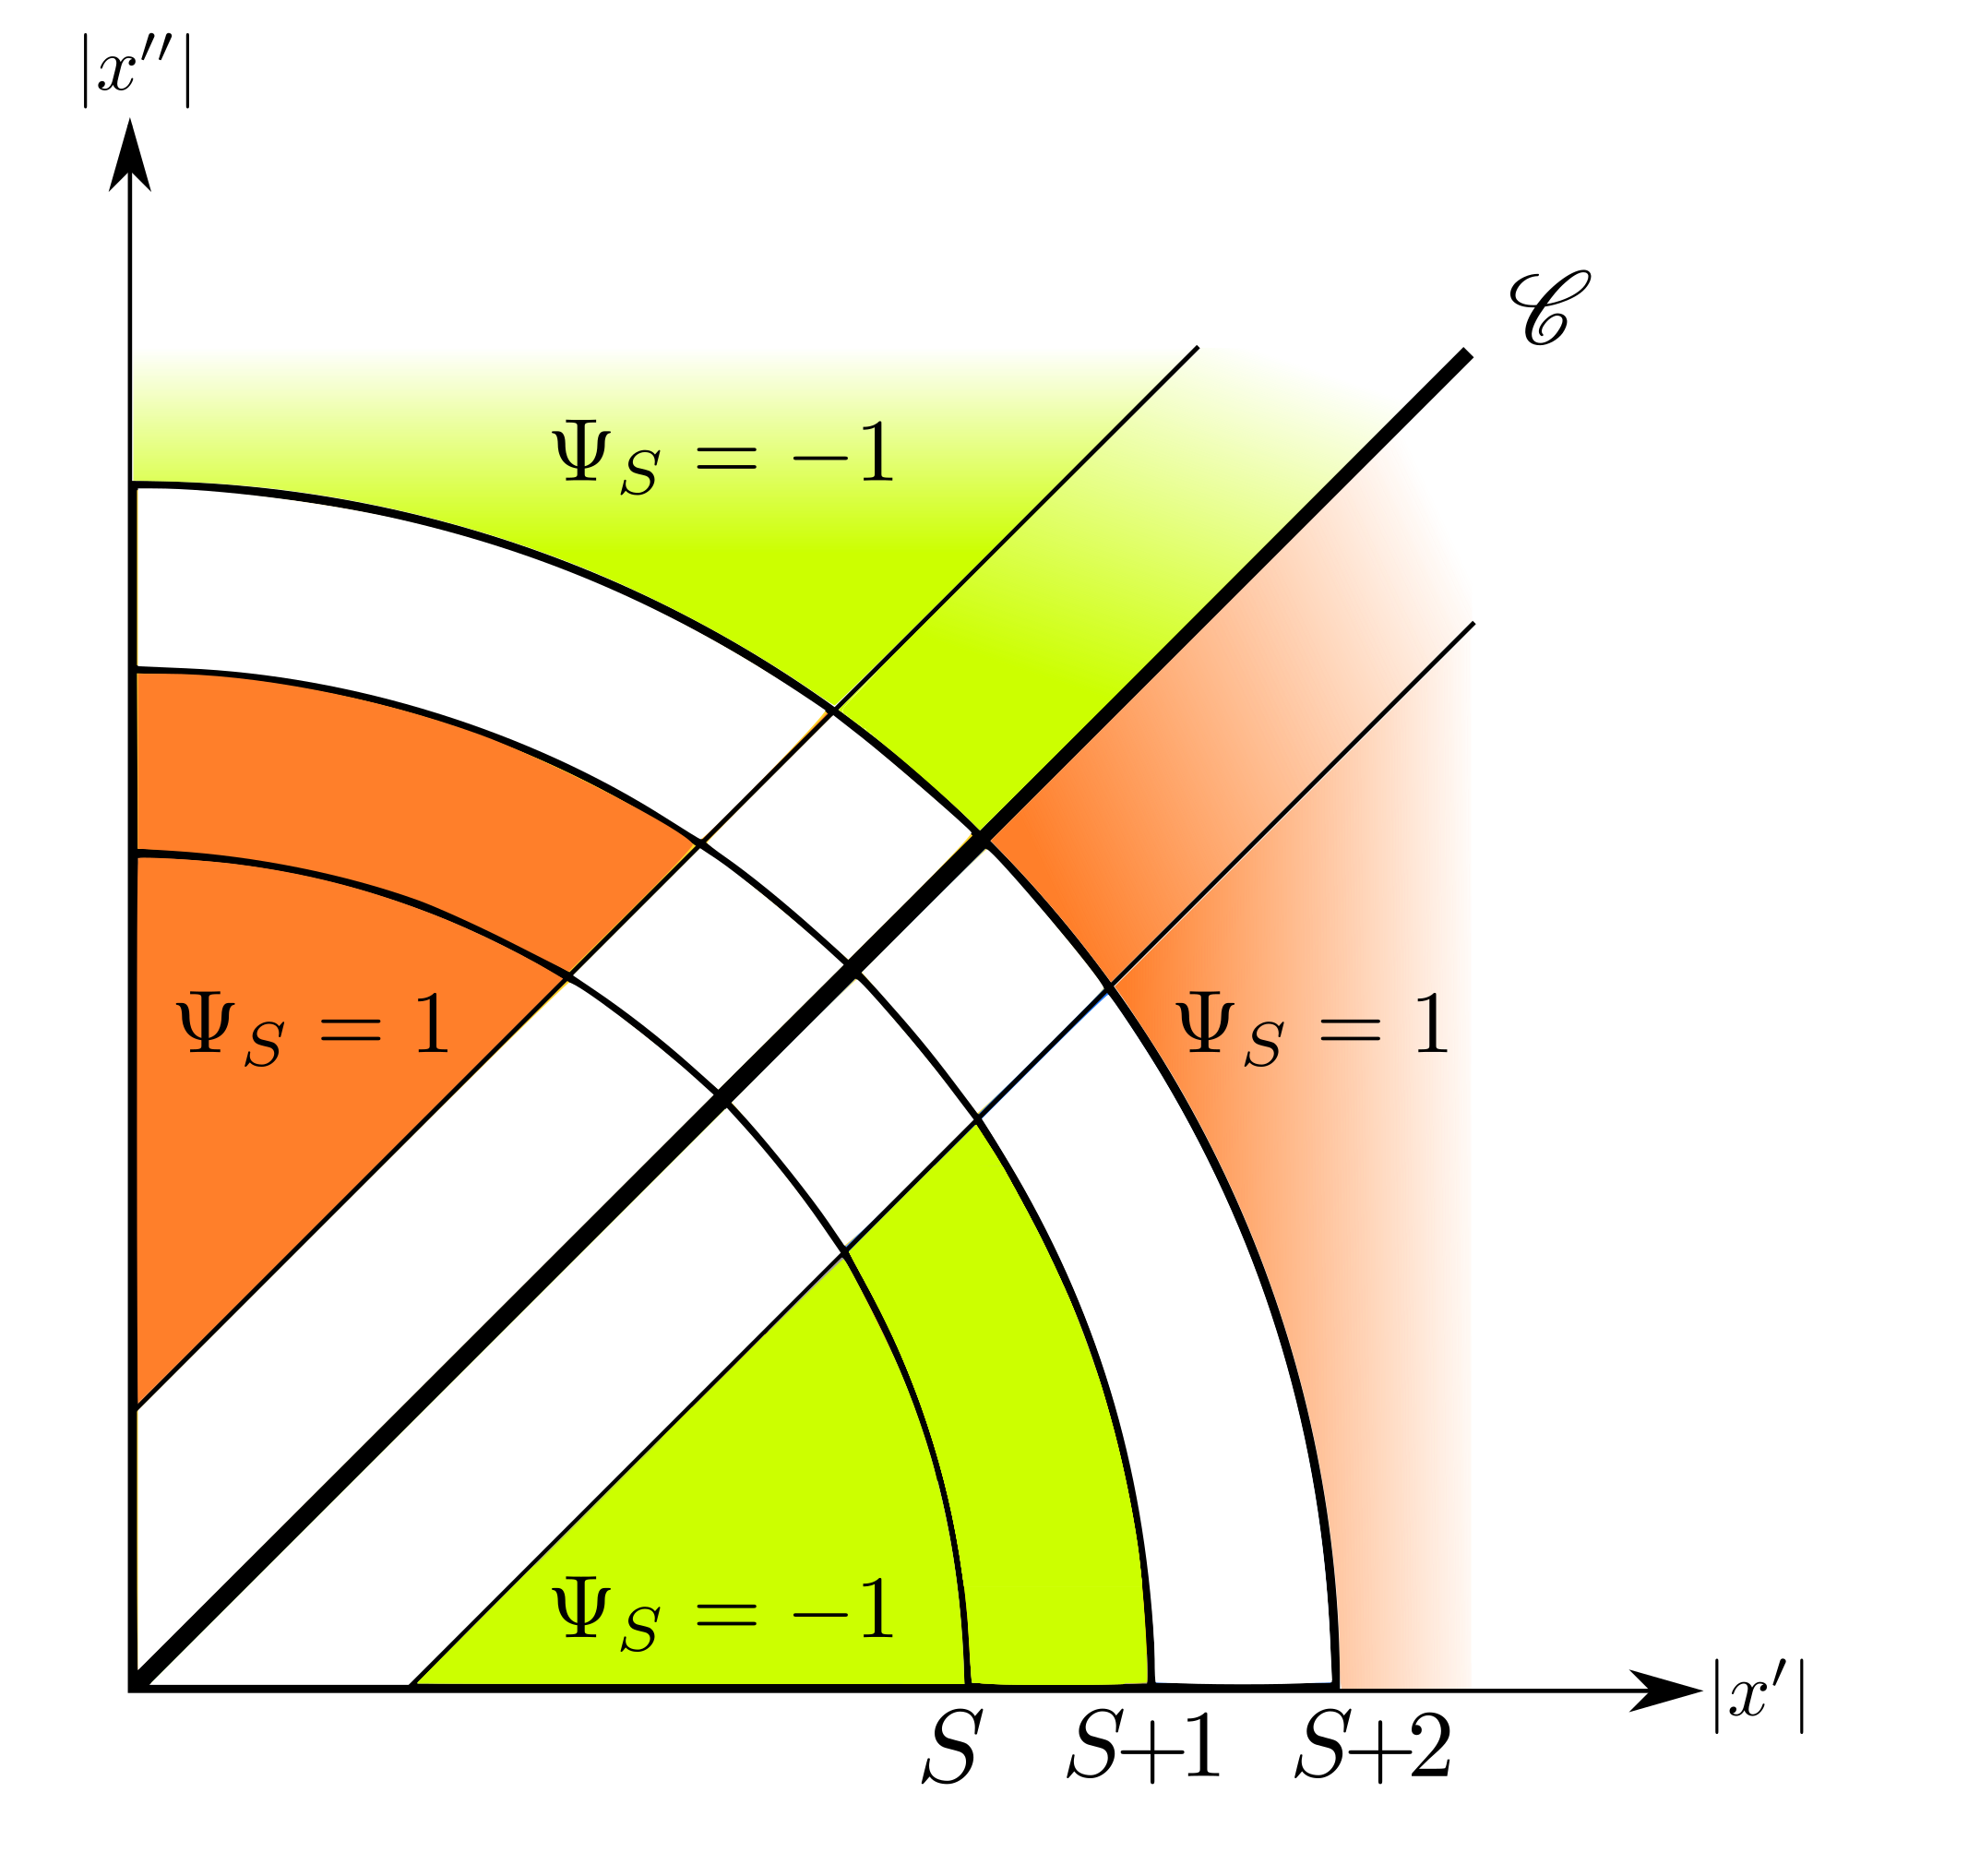
\includegraphics[width = \textwidth]{EnergyEstimatePsiS.png}
	\end{subfigure}
	\begin{subfigure}{0.49\textwidth}
		\centering
		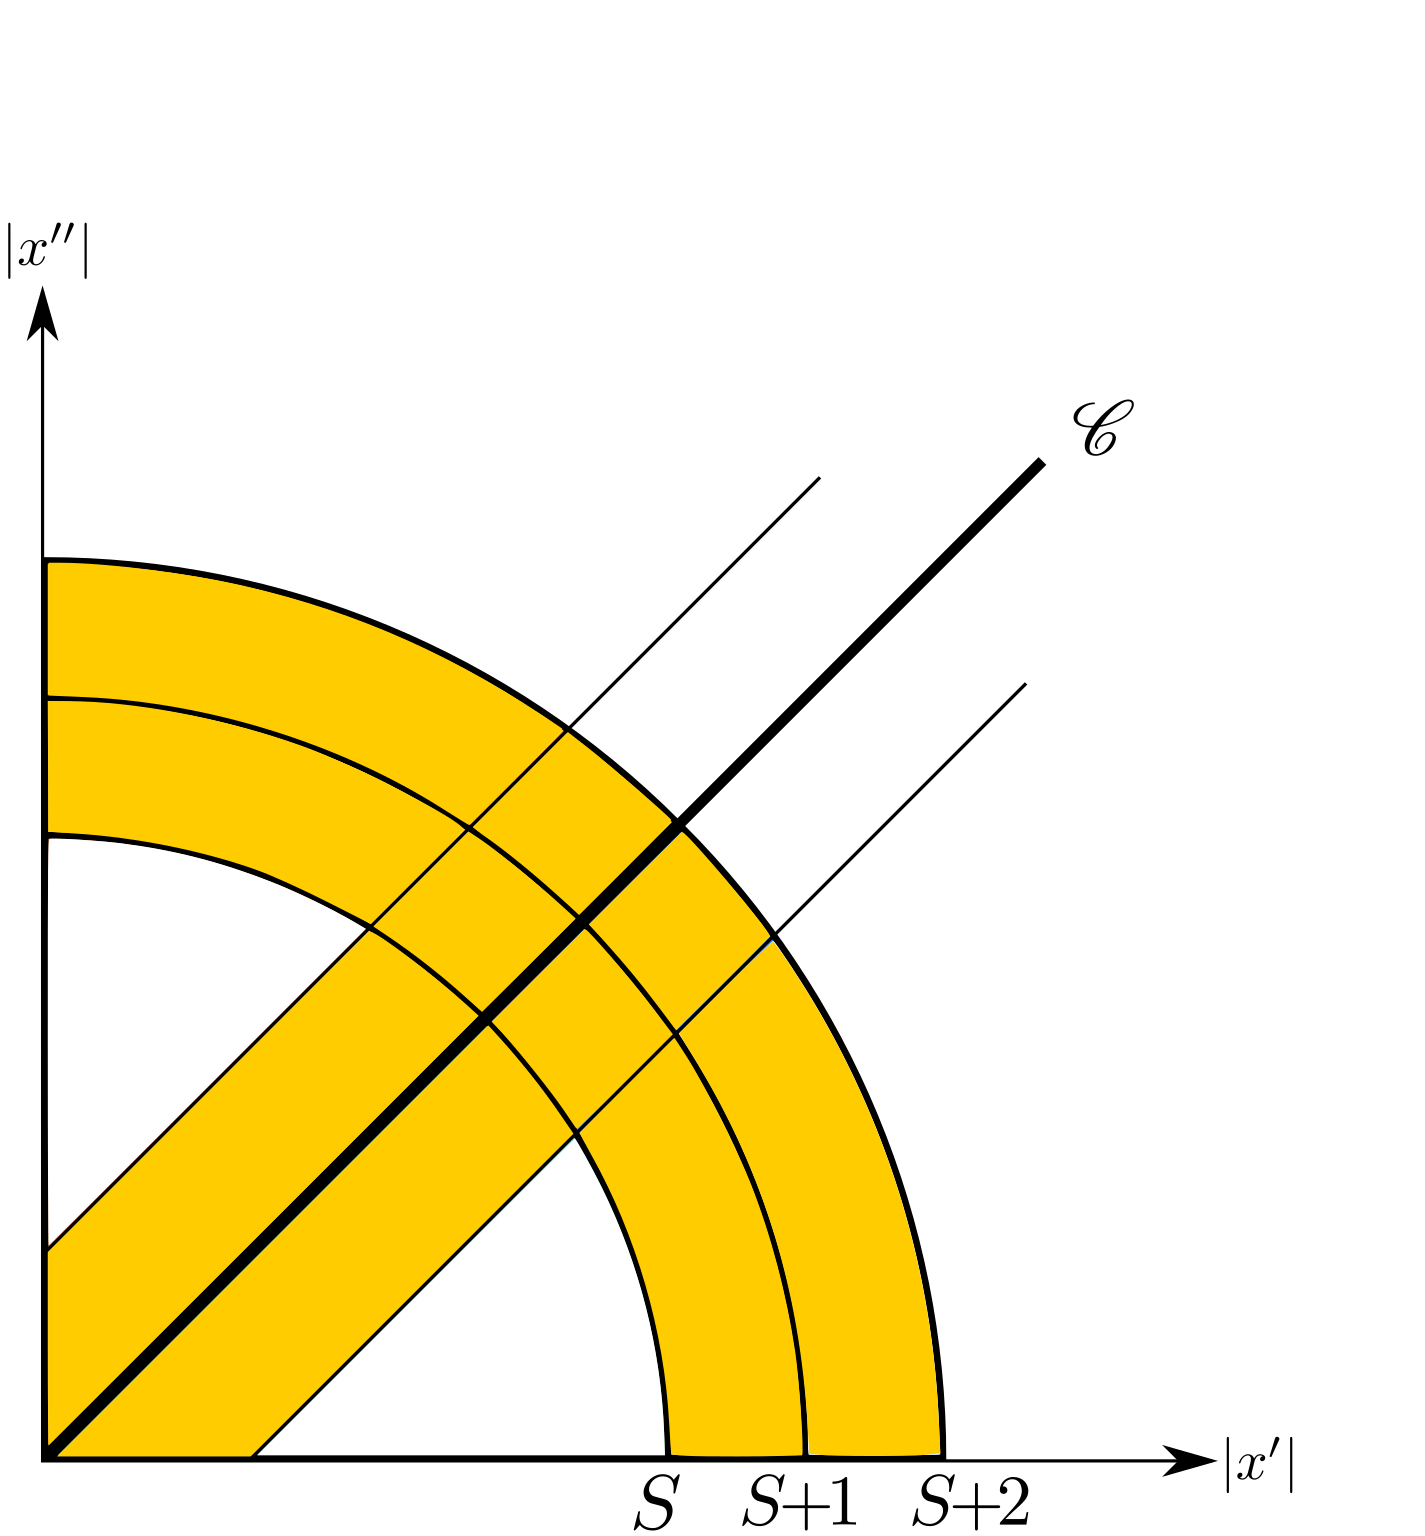
\includegraphics[width = \textwidth]{EnergyEstimateOmegaS.png}
	\end{subfigure}
	\caption{(a) The $1$ and $-1$ level sets of $\Psi_S$. (b) The set $\Omega_S$.}
	\label{Fig:PsiSandOmegaS}
\end{figure}

Note that both $\Psi_S$ and $d_S$ are Lipschitz functions, with Lipschitz norm independent of
$S$. Moreover $\Psi_S$ is odd and $d_S$ even with respect to the Simons cone. Regarding the set $\overline{\Omega_S}$, we can see it as the preimage of $1$ through $d_S$ inside $\overline{B_{S+2}}$.

Now we show some auxiliary results concerning the previous definitions.

\begin{lemma}
\label{Lemma: AdaptedLipschitzConditionWith_dFunction}
Given $S>0$, if either $(x,y) \in \left(\Omega_S\cap \ocal\right) \times \ical$ or $(x,y)\in \left(B_{S+2}\cap \ocal\right) \times \ocal$, then
$$ |\Psi_S(x) - \Psi_S(y)| \leq C \frac{|x-y|}{d_S(x)} \ \ \ \ \ \textrm{whenever} \ \ |x-y|\leq d_S(x), $$
with $C>0$ independent of $S$.
\end{lemma}

\begin{proof}
Note first that if $x\in \Omega_S \cap \ocal$, then $d_S(x)=1$ and the result is trivial by the Lipschitz continuity of $\Psi_S$. Hence, we only need to establish the result for the case $x\in B_S\cap \{\dist(x,\ccal)\geq 1\} \cap \ocal$ and $y\in \ocal$. Under these hypotheses, we have that $\Psi_S(x)=-1$ and $d_S(x) = \min\{S+1-|x|,\dist(x,\ccal)\}$. Moreover, since $x\in B_S$ and $\dist(x,\ccal)\geq 1$ we get $d_S(x) \leq S+1-|x|$. Therefore, if $|x-y|\leq d_S(x)$ we obtain
$$ |y|\leq |x-y| + |x| \leq d_S(x)+|x| \leq S+1. $$

Now we distinguish two cases, either $\{\dist(\cdot,\ccal)\geq 1\}$ or $\{\dist(\cdot,\ccal)\leq 1\}$. Assume first that $y\in B_{S+1} \cap \{\dist(\cdot,\ccal)\geq 1\}\cap \ocal$. Then, $\Psi_S(y)=-1$ and the result is trivial from being also $\Psi_S(x)=-1$. Thus, it only remains to show the result in the case $x\in B_S \cap \{\dist(\cdot,\ccal)\geq 1\}\cap \ocal$ and $y\in B_{S+1} \cap \{\dist(\cdot,\ccal)\leq 1\}\cap \ocal$. Note that under these assumptions, $\Psi_S(x)=-1$ and $\Psi_S(y)=-\dist(y,\ccal)$.


Given $x,y \in \R^{2m}$ it is easy to prove by using the triangular inequality and the definition of distance to the cone that
\begin{equation} \label{Eq:TriangularCone}
\dist(x,\ccal) \leq |x-y| + \dist(y,\ccal).
\end{equation}
Therefore we have
\begin{equation} \label{Eq:TriangularCone2}
1-|x-y|-\dist(y,\ccal) \leq 1-\dist(x,\ccal) \leq 0
\end{equation}
Now, multiplying \eqref{Eq:TriangularCone} by $|1-\dist(y,\ccal)|$ and using \eqref{Eq:TriangularCone2} we obtain
\begin{align*}
|1-\dist(y,\ccal)|\,\dist(x,\ccal) &\leq |1-\dist(y,\ccal)| \left(|x-y| + \dist(y,\ccal)\right) \\
%&= \left(1-\dist(y,\ccal)\right) \left(|x-y| + \dist(y,\ccal)\right) \\
&= |x-y|+\dist(y,\ccal) \left\{ -|x-y|+ 1- \dist(y,\ccal) \right\} \\
&\leq |x-y|.
\end{align*}

Hence,
$$ |\Psi_S(x)-\Psi_S(y)| = |1-\dist(y,\ccal)| \leq \frac{|x-y|}{\dist(x,\ccal)} \leq  \frac{|x-y|}{d_S(x)},$$
completing the proof.
\end{proof}

Another auxiliary result that we will need in the proof of Theorem~\ref{Th:EnergyEstimate} is the following estimate for the function $d_S$. 

\begin{lemma}
\label{Lemma:Integrability_dFunction}
Given $S>0$ we have
$$ \int_{B_{S+2}} d_S(x)^{-2\s} \d x \leq \begin{cases}
C \ S^{2m-2\s}\ \ \ \ &\textrm{if } \ \ \s\in(0,1/2),\\
C\ \log(S)\,S^{2m-2\s}\ \ \ \ &\textrm{if } \ \ \s=1/2,\\
C \ S^{2m-1}\ \ \ \ &\textrm{if } \ \ \s\in(1/2,1),\\
\end{cases} $$
with $C>0$ independent of $S$ and only depending on $m$ and $\s$.
\end{lemma}

\begin{proof}
In order to prove this result we first note that $d_S(x)=1$ in $\Omega_S$. Thus, the contribution to the integral of this part is just its measure, which is well known to be of order $2m-1$ (see the proof of the energy estimate in \cite{CabreTerraI}). That is,
$$\int_{\Omega_S} d_S(x)^{-2\s} \d x = |\Omega_S| \leq C\,S^{2m-1}.$$

For the other part of the integral we can write
\begin{align*}
\int_{B_{S+2}\setminus \Omega_S} d_S(x)^{-2\s} \d x &= \int_{B_{S}\cap \dist\{x,\ccal\}>1} d_S(x)^{-2\s} \d x \\
& \leq \int_{B_{S}\cap \dist\{x,\ccal\}>1} \left( S+1-|x| \right)^{-2\s} \d x + \int_{B_{S}\cap \dist\{x,\ccal\}>1} \dist(x,\ccal)^{-2\s} \d x.
\end{align*}
The desired estimate for the first integral can be found in \cite{SavinValdinoci-EnergyEstimate}. Therefore, in order to complete the proof it only remains to estimate the second integral. It can be estimated by writing it in $(y,z)$ variables, where
$$
y = \dfrac{|x'|+|x''|}{\sqrt{2}} \, \quad \text{ and } z = \dfrac{|x'|-|x''|}{\sqrt{2}}\,.
$$
In this case, $z$ is the signed distance to the cone. Thus,
\begin{align*}
\int_{B_{S}\cap \dist\{x,\ccal\}>1} \dist(x,\ccal)^{-2\s} \d x &\leq C \int \int_{B_{S}\cap \{y\geq|z|>1\}} |z|^{-2\s} \, (y^2-z^2)^{m-1} \d y\d z \\
& \leq C \int \int_{B_{S}\cap \{y\geq|z|>1\}} |z|^{-2\s} \, y^{2m-2} \d y\d z \\
& \leq C\, \int_1^S \d z \int_0^S \d y\ z^{-2\s} \, y^{2m-2} \\
& \leq C\, \left(\int_1^S z^{-2\s} \d z \right)  \left(  \int_0^S \d y \, y^{2m-2} \right) \\
& \leq \begin{cases}
C \ S^{2m-2\s}\ \ \ \ &\textrm{if } \ \ \s\in(0,1/2),\\
C\ \log(S)\,S^{2m-2\s}\ \ \ \ &\textrm{if } \ \ \s=1/2,\\
C \ S^{2m-1}\ \ \ \ &\textrm{if } \ \ \s\in(1/2,1).\\
\end{cases}
\end{align*}
\end{proof}


The last auxiliary result we need in order to establish the energy estimate is the following inequality.

\begin{lemma}
\label{Lemma: InteractionInequalityMinimumFunction}
Let $A\subset B_R \subset \R^{2m}$ be a set of double revolution such that $A^\star = A$ and let $\omega, \phi, \varphi \in \widetilde{\H}^K(B_R)$ be such that
$$\begin{cases}
\omega = \phi \leq \varphi \ \ \ \ \textrm{in } \ \ \ \ocal \setminus A\,,\\
\omega = \varphi \leq \phi \ \ \ \ \textrm{in } \ \ \ \ocal \cap A\,.
\end{cases}$$
Then, if $K$ satisfies \eqref{Eq:KernelInequalityReflexion}, it holds
\begin{align*}
I_\omega(\ocal\cap A, \ocal \setminus A) \leq I_\phi(\ocal\cap A, \ocal \setminus A) + I_\varphi(\ocal\cap A, \ocal \setminus A)\,,
\end{align*}
where $I_w(\cdot, \cdot)$ is the interaction defined in \eqref{Eq:DefIw}.
\end{lemma}

\begin{proof}
A simple computation shows that if $x\in \ocal \cap A$ and $y\in \ocal \setminus A$ we have that
$$ |\phi(x)-\phi(y)|^2+|\varphi(x)-\varphi(y)|^2\geq |\omega(x)-\omega(y)|^2. $$
Indeed,
\begin{align*}
|\phi(x)-\phi(y)|^2+|\varphi(x)&-\varphi(y)|^2 - |\omega(x)-\omega(y)|^2 \\
&= |\phi(x)-\phi(y)|^2+|\varphi(x)-\varphi(y)|^2 - |\varphi(x)-\phi(y)|^2 \\
&= \phi^2(x)-2\phi(x)\phi(y)+\varphi^2(y)-2\varphi(x)\varphi(y)+2\varphi(x)\phi(y) \\
&= \left( \phi(x) - \varphi(y)\right) ^2+2\left( \phi(x)-\varphi(x) \right) \left( \varphi(y)-\phi(y) \right) \\
&\geq 0.
\end{align*}
Therefore, by using this inequality and the reflexion property of the kernel, \eqref{Eq:KernelInequalityReflexion}, we obtain
\begin{align*}
I_\phi(\ocal\cap A, \ocal \setminus A) &+ I_\varphi(\ocal\cap A, \ocal \setminus A) - I_\omega(\ocal\cap A, \ocal \setminus A) = \\
&\hspace{-26mm}= \int_{\ocal\cap A} \d x \int_{\ocal\setminus A} \d y \left\{|\phi(x)-\phi(y)|^2+|\varphi(x)-\varphi(y)|^2-|\omega(x)-\omega(y)|^2 \right\} \left\{\overline{K}(x,y)-\overline{K}(x,y^\star)\right\} \\
&\hspace{-20mm}+ 2 \int_{\ocal\cap A} \d x \int_{\ocal\setminus A} \d y \left\{\phi^2(x)+\phi^2(y)+\varphi^2(x)+\varphi^2(y)-\omega^2(x)-\omega^2(y) \right\} \overline{K}(x,y^\star) \\
&\hspace{-26mm}\geq 2\int_{\ocal\cap A} \d x \int_{\ocal\setminus A} \d y \left\{
\phi^2(x)+\varphi^2(y)\right\} \overline{K}(x,y^\star) \geq 0.
\end{align*}
\end{proof}



With all these ingredients we can establish now the sharp energy estimate.

\begin{proof}[Proof of Theorem~\ref{Th:EnergyEstimate}]

Note that, by Lemma~\ref{Lemma:DecreaseEnergy}  we can assume without loss of generality that if $u$ is a minimizer of $\ecal$ in $B_R$, then $-1 \leq u \leq 1$, $u \geq 0$ in $\ocal$, and $u \leq 0$ in $\ical$. 

\textbf{Step 1. We show that $0\leq u < 1$ in $\ocal$.} 

In order to prove it we first need to show that $u$ is a weak solution of
\begin{equation}
\label{Eq:ProofEnergyEstimateProblemBR}
	\beqc{\PDEsystem}
	L u &=& f(u) & \textrm{ in } B_R\,,\\
	u &=& 0 & \textrm{ in }\R^{2m} \setminus B_R.
	\eeqc
\end{equation}
To see this, we consider on the one hand perturbations $u +  \varepsilon \xi$, with $\xi \in \widetilde{\H}^K_{0, \,\mathrm{odd}}(B_R)$ and such that $\xi$ has compact support in $B_R$. Then, since $u$ is a minimizer among functions in $\widetilde{\H}^K_{0, \,\mathrm{odd}}(B_R)$, we get
$$
0 = \dfrac{\d}{\d \varepsilon}\evalat{\varepsilon = 0} \ecal(u +  \varepsilon \xi, B_R) = \langle u,\xi \rangle_{\widetilde{\H}^K_0(B_R)} - \langle f(u),\xi \rangle_{L^2(B_R)}\,.
$$
On the other hand, take $\xi \in \widetilde{\H}^K_{0, \,\mathrm{even}}(B_R)$. Since $u$ is odd with
respect to the Simons cone, so is $f(u)$. Then, by Remark~\ref{Remark:DecompositionHK} and the same
decomposition in $L^2(B_R)$, we find that
$$
\langle v_R,\xi \rangle_{\widetilde{\H}^K_0(B_R)} = 0 \quad \textrm{ and } \quad  \langle f(v_R),\xi \rangle_{L^2(B_R)} = 0\,.
$$
Therefore, we have that
$$
\langle u,\xi \rangle_{\widetilde{\H}^K_0(B_R)} = \langle f(u),\xi \rangle_{L^2(B_R)}
$$
for every $\xi \in\widetilde{\H}^K_0(B_R)$ with compact support in  $B_R$. Thus,
$$
\int_{\R^{2m}}\int_{\R^{2m}} \{u(x)-u(y)\}\{\xi(x)-\xi(y)\} K(|x-y|) \d x \d y = \int_{\R^{2m}} f(u(x)) \xi(x) \d x
$$
for every $\xi \in C^\infty_0(\Omega)$ that is double radially symmetric. 

By Proposition~\ref{Prop:WeakSolutionForAllTestFunctions}, $u$ is a weak solution of \eqref{Eq:ProofEnergyEstimateProblemBR}, and by the regularity result of Corollary \ref{Cor:C2regularity}, since $u$ is bounded, it is a classical solution.

From being $u$ a classical solution it is easy to show that it cannot be $1$ or $-1$ and therefore that it satisfies $0\leq u < 1$ in $\ocal$. That is, let us suppose that there exists $x_0\in\R^{2m}$ such that $|u(x_0)|=1$. It is clear that we can take $x_0\in\ocal\cap B_R$. Then, from equation \eqref{Eq:ProofEnergyEstimateProblemBR} and the fact of being $x_0$ an absolute maximum, we can arrive at a contradiction:
\begin{align*}
0 &= f(1) = f(u(x_0)) = Lu(x_0) = \int_\ocal (1-u(y)) \overline{K}(x,y) + (1+u(y)) \overline{K}(x,y^\star)  \d y \\
&\geq \int_\ocal (1-u(y)) \overline{K}(x,y^\star) + (1+u(y)) \overline{K}(x,y^\star)  \d y = 2\int_\ocal \overline{K}(x,y^\star) \d y\\
&>0.
\end{align*}

\textbf{Step 2. We build a suitable competitor for $u$ and compare their energies.}

Now, for $x\in \ocal$ we define
$$ 
v(x) := \min\{u(x),\Psi_S(x)\}, 
$$
and we define it in $\ical$ by considering its odd reflection with respect to the Simons cone. Let us also define
$$
A = \{v=\Psi_S\} = \{\Psi_S \leq u\}. 
$$
Then, it is easy to check that we have the inclusions
\begin{equation}
\label{Eq:EnergyEstimateProofInclusionsA}
	B_{S+1} \subset A \subset B_{S+2}\,.
\end{equation}
To do it, note first that we only need to prove it inside $\ocal$, by the symmetry of $A$ with respect to the Simons cone. On the one hand, if $ x\in B_{S+1}\cap \ocal$, then $\Psi_S(x) = \max\{-1,-\dist(x,\ccal)\} \leq 0 \leq u(x)$, which yields $v(x) = \Psi_S(x)$ Thus, $x\in A\cap \ocal$. On the other hand, if $ x\in A\cap \ocal$ then $\Psi_S(x) \leq u(x) < 1$. This can only happen if $x\in B_{S+2}$.

Note that both $u$ and $v$ are equal outside $B_{S+2} \subset B_R$, and therefore $v$ is an admissible competitor. By comparing the energies of $u$ and $v$ we will obtain the desired estimate. 

Let us decompose the energy of $u$ in $B_R$ in terms of interactions between sets that involve $A$. That is,
\begin{align*}
\ecal(u,B_R) &= \frac{1}{2}I_u(\ocal \cap A, \ocal \cap A) + I_u(\ocal \cap A, \ocal \setminus A) \\
& \hspace{5mm} + \frac{1}{2}I_u\big((\ocal \setminus A) \cap B_R, (\ocal \setminus A) \cap B_R\big) + I_u\big((\ocal \setminus A) \cap B_R, \ocal \setminus B_R\big) \\
& \hspace{5mm} + \int_A G(u) + \int_{B_R\setminus A} G(u)
\end{align*}
Since $u$ is a minimizer, $v=\Psi_S$ in $A$ and $u=v$ outside of $A$,  from the previous expression we obtain
\begin{align*}
0 &\leq \ecal(v,B_R)-\ecal(u,B_R) = \frac{1}{2}I_{\Psi_S}(\ocal \cap A, \ocal \cap A) - \frac{1}{2}I_u(\ocal \cap A, \ocal \cap A)\\
& \hspace{5mm} + I_v(\ocal \cap A, \ocal \setminus A) - I_u(\ocal \cap A, \ocal \setminus A) + \int_A G(\Psi_S) - \int_{A} G(u)
\end{align*}
Since $v = \min\{u,\Psi_S\}$ in $\ocal$ we can apply Lemma \ref{Lemma: InteractionInequalityMinimumFunction} with $\omega = v$, $\Psi_S = \varphi$, and $u= \phi$, to get
\begin{align*}
\frac{1}{2}I_u(\ocal \cap A, \ocal \cap A) + \int_{A} G(u) &\leq \frac{1}{2}I_{\Psi_S}(\ocal \cap A, \ocal \cap A) + I_{\Psi_S}(\ocal \cap A, \ocal \setminus A) + \int_A G(\Psi_S)  \\
&= \ecal(\Psi_S, A) \leq \ecal(\Psi_S,B_{S+2})
\end{align*}
From this and using \eqref{Eq:EnergyEstimateProofInclusionsA}, we deduce an estimate for the energy of $u$ in $B_S$ as follows.
\begin{align*}
\ecal(u,B_S) &\leq \frac{1}{2}I_u(\ocal \cap A, \ocal \cap A) + \int_{A} G(u) + I_u(\ocal \setminus B_{S+1}, \ocal \cap B_S) \\
& \leq  \ecal(\Psi_S,B_{S+2}) + I_u(\ocal \setminus B_{S+1}, \ocal \cap B_S).
\end{align*}
Thus, to obtain the desired energy estimate we only have to bound the right-hand side of the last inequality.


\textbf{Step 3. We estimate the remaining terms.}

In the following arguments, we use the definition of the energy that involves the original kernel $K$ and not $\overline{K}$.

\textbf{3.1. Estimate for $\ecal(\Psi_S,B_{S+2})$.}
First, by using the change of variables given by $(\cdot)^\star$ and the ellipticity of $K$, \eqref{Eq:Ellipticity}, we obtain
\begin{align*}
\ecal(\Psi_S,B_{S+2}) &= \frac{1}{4} \int_{B_{S+2}} \int_{B_{S+2}} |\Psi_S(x)-\Psi(y)|^2K(|x-y|) \d x\d y \\
&\hspace{5mm} +\frac{1}{2} \int_{B_{S+2}} \int_{\R^{2m} \setminus B_{S+2}} |\Psi_S(x)-\Psi(y)|^2K(|x-y|) \d x\d y + \int_{B_{S+2}} G(\Psi_S) \\
&\leq \frac{1}{2} \int_{B_{S+2}} \int_{\R^{2m}} |\Psi_S(x)-\Psi(y)|^2K(|x-y|) \d x\d y + \int_{B_{S+2}} G(\Psi_S) \\
&= \int_{B_{S+2} \cap \ocal} \int_{\R^{2m}} |\Psi_S(x)-\Psi(y)|^2K(|x-y|) \d x\d y + \int_{B_{S+2}} G(\Psi_S) \\
&= \Lambda \int_{B_{S+2} \cap \ocal} \int_{\R^{2m}} \frac{|\Psi_S(x)-\Psi(y)|^2}{|x-y|^{n+2\s}} \d x\d y + \int_{B_{S+2}} G(\Psi_S).
\end{align*}
Now, we split the domain of integration of the kinetic energy into three parts.
\begin{align*}
\ecal(\Psi_S,B_{S+2}) &\leq \Lambda \int_{B_{S+2} \cap \ocal} \int_{\ocal} \frac{|\Psi_S(x)-\Psi(y)|^2}{|x-y|^{n+2\s}} \d x\d y \\
&\hspace{5mm} + \Lambda \int_{\Omega_S \cap \ocal} \int_{\ical} \frac{|\Psi_S(x)-\Psi(y)|^2}{|x-y|^{n+2\s}} \d x\d y \\
&\hspace{5mm} + \Lambda \int_{(B_{S+2}\setminus \Omega_S) \cap \ocal} \int_{\ical} \frac{|\Psi_S(x)-\Psi(y)|^2}{|x-y|^{n+2\s}} \d x\d y + \int_{B_{S+2}} G(\Psi_S) \\
&=:I_1+I_2+I_3+I_G,
\end{align*}
where $\Omega_S$ is defined in \eqref{Eq:DefOmegaS}. 

Let us estimate this four integrals. 
\begin{align*}
I_1 &= \Lambda \int_{B_{S+2} \cap \ocal} \int_{\ocal} \frac{|\Psi_S(x)-\Psi(y)|^2}{|x-y|^{n+2\s}} \d x\d y\\
&= \Lambda \int_{B_{S+2} \cap \ocal} \int_{\ocal\cap\{|x-y|\leq d_S(x)\}} \frac{|\Psi_S(x)-\Psi(y)|^2}{|x-y|^{n+2\s}} \d x\d y\\
&\hspace{5mm} + \Lambda \int_{B_{S+2} \cap \ocal} \int_{\ocal\cap\{|x-y|\geq d_S(x)\}} \frac{|\Psi_S(x)-\Psi(y)|^2}{|x-y|^{n+2\s}} \d x\d y\\
&\leq C \int_{B_{S+2} \cap \ocal} d_S(x)^{-2}\int_{\ocal\cap\{|x-y|\leq d_S(x)\}} |x-y|^{2-n-2\s} \d y\d x\\
&\hspace{5mm} + C \int_{B_{S+2} \cap \ocal} \int_{\ocal\cap\{|x-y|\geq d_S(x)\}} |x-y|^{-n-2\s} \d x\d y\\
&\leq C \int_{B_{S+2} \cap \ocal} d_S(x)^{-2}\int_0^{d_S(x)} \rho^{1-2\s} \d \rho\d x + C \int_{B_{S+2} \cap \ocal}  \int_{d_S(x)}^\infty \rho^{-1-2\s} \d\rho \d x\\
&\leq C \int_{B_{S+2} \cap \ocal} d_S(x)^{-2\s} \d x,
\end{align*}
where in the first inequality we have used Lemma~\ref{Lemma: AdaptedLipschitzConditionWith_dFunction} and the uniform bound of $\Psi_S$. The bound of $I_2$ is essentially the same using also Lemma~\ref{Lemma: AdaptedLipschitzConditionWith_dFunction} and the inclusion $\Omega_S \subset B_{S+2}$. That is,
\begin{align*}
I_2 &= \Lambda \int_{\Omega_S \cap \ocal} \int_{\ical} \frac{|\Psi_S(x)-\Psi(y)|^2}{|x-y|^{n+2\s}} \d x\d y\\
&= \Lambda \int_{\Omega_S \cap \ocal} \int_{\ical\cap\{|x-y|\leq d_S(x)\}} \frac{|\Psi_S(x)-\Psi(y)|^2}{|x-y|^{n+2\s}} \d x\d y\\
&\hspace{5mm} + \Lambda \int_{\Omega_S \cap \ocal} \int_{\ical\cap\{|x-y|\geq d_S(x)\}} \frac{|\Psi_S(x)-\Psi(y)|^2}{|x-y|^{n+2\s}} \d x\d y\\
&\leq C \int_{\Omega_S \cap \ocal} d_S(x)^{-2}\int_0^{d_S(x)} \rho^{1-2\s} \d \rho\d x + C \int_{\Omega_S \cap \ocal}  \int_{d_S(x)}^\infty \rho^{-1-2\s} \d\rho \d x\\
&\leq C \int_{\Omega _S\cap \ocal} d_S(x)^{-2\s} \d x \leq C \int_{B_{S+2} \cap \ocal} d_S(x)^{-2\s} \d x.
\end{align*}
For the case of $I_3$, we use the fact that given $x\in (B_{S+2}\setminus \Omega_S)\cap \ocal$, then $\dist(x,\ccal)\geq d_S(x)$ and therefore $\ical \subset \R^{2m}\setminus B_{d_S(x)}(x)$.
\begin{align*}
I_3 &= \Lambda \int_{(B_{S+2}\setminus \Omega_S) \cap \ocal} \int_{\ical} \frac{|\Psi_S(x)-\Psi(y)|^2}{|x-y|^{n+2\s}} \d x\d y \leq C \int_{(B_{S+2}\setminus \Omega_S) \cap \ocal} \int_{\R^{2m}\setminus B_{d_S(x)}(x)} |x-y|^{-n-2\s} \\
&\leq C \int_{B_{S+2} \cap \ocal} \int_{d_S(x)}^\infty \rho^{-1-2\s} \d \rho\d x \leq C \int_{B_{S+2} \cap \ocal} d_S(x)^{-2\s} \d x.
\end{align*}
Finally, we estimate $I_G$. Since $\Psi_S$ is either $1$ or $-1$ in $B_{S+2}\setminus \Omega_S$, and $G(-1)=G(1)=0$, we have
\begin{align*}
I_G = \int_{B_{S+2}} G(\Psi_S) = \int_{\Omega_S} G(\Psi_S) \leq C | \Omega_S| \leq C\,S^{2m-1}\,.
\end{align*}
Therefore, we obtain
\begin{align*}
\ecal(\Psi_S,B_{S+2}) &\leq C \left(\int_{B_{S+2} \cap \ocal} d_S(x)^{-2\s} \d x + S^{2m-1} \right)\leq C\left(\int_{B_{S} \cap \ocal} d_S(x)^{-2\s} \d x + S^{2m-1} \right).
\end{align*}

%%%%%%%%%

\textbf{3.2. Estimate for $I_u(\ocal \setminus B_{S+1}, \ocal \cap B_S)$.} First, we claim that $|x-y|\geq d_S(x)$ whenever $x\in B_S\cap \ocal$ and $y\in \R^{2m}\setminus B_{S+1}$. Indeed, if $x\in B_S$, then $d_S(x) \leq S+1-|x|$ and therefore we have $|x-y|\geq |y|-|x|\geq |y|+d_S(x)-S-1 \geq  d_S(x)$, since $|y| \geq S+1$. Thus, using this and the ellipticity of $K$ we get
\begin{align*}
I_u(\ocal \setminus B_{S+1}, \ocal \cap B_S) &\leq C \int_{B_S \cap \ocal} \d x \int_{\R^{2m}\setminus B_{S+1}} \d y \ \frac{|u(x)-u(y)|^2}{|x-y|^{2m+2\s}} \\
& C \leq \int_{B_S \cap \ocal} \d x \int_{|x-y|\geq d_S(x)} \d y \ |x-y|^{-2m-2\s} \\
&\leq C \int_{B_S \cap \ocal} d_S(x)^{-2\s} \d x.
\end{align*}

\textbf{Step 4. Conclusion.}

Finally, by adding up the estimates of Step~3 and applying Lemma~\ref{Lemma:Integrability_dFunction}, we obtain the desired result. That is,
\begin{align*}
\ecal(u,B_S) &\leq \ecal(\Psi_S,B_{S+2}) + I_u(\ocal \setminus B_{S+1}, \ocal \cap B_S) \leq C\left(\int_{B_S \cap \ocal} d_S(x)^{-2\s} \d x + S^{2m-1} \right)\\
&\leq \begin{cases}
C \ S^{2m-2\s}\ \ \ &\textrm{if } \ \ \s\in(0,1/2),\\
C\ \log(S)\,S^{2m-2\s}\ \ \ \ &\textrm{if } \ \ \s=1/2,\\
C \ S^{2m-1}\ \ \ \ &\textrm{if } \ \ \s\in(1/2,1).\\
\end{cases}
\end{align*}
\end{proof}
